\documentclass[nooutcomes,noauthor,hints]{ximera}

\graphicspath{  
{./}
{./whoAreYou/}
{./drawingWithTheTurtle/}
{./bisectionMethod/}
{./circles/}
{./anglesAndRightTriangles/}
{./lawOfSines/}
{./lawOfCosines/}
{./plotter/}
{./staircases/}
{./pitch/}
{./qualityControl/}
{./symmetry/}
{./nGonBlock/}
}


%% page layout
\usepackage[cm,headings]{fullpage}
\raggedright
\setlength\headheight{13.6pt}


%% fonts
\usepackage{euler}

\usepackage{FiraMono}
\renewcommand\familydefault{\ttdefault} 
\usepackage[defaultmathsizes]{mathastext}
\usepackage[htt]{hyphenat}

\usepackage[T1]{fontenc}
\usepackage[scaled=1]{FiraSans}

%\usepackage{wedn}
\usepackage{pbsi} %% Answer font


\usepackage{cancel} %% strike through in pitch/pitch.tex


%% \usepackage{ulem} %% 
%% \renewcommand{\ULthickness}{2pt}% changes underline thickness

\tikzset{>=stealth}

\usepackage{adjustbox}

\setcounter{titlenumber}{-1}

%% journal style
\makeatletter
\newcommand\journalstyle{%
  \def\activitystyle{activity-chapter}
  \def\maketitle{%
    \addtocounter{titlenumber}{1}%
                {\flushleft\small\sffamily\bfseries\@pretitle\par\vspace{-1.5em}}%
                {\flushleft\LARGE\sffamily\bfseries\thetitlenumber\hspace{1em}\@title \par }%
                {\vskip .6em\noindent\textit\theabstract\setcounter{question}{0}\setcounter{sectiontitlenumber}{0}}%
                    \par\vspace{2em}
                    \phantomsection\addcontentsline{toc}{section}{\thetitlenumber\hspace{1em}\textbf{\@title}}%
                     }}
\makeatother



%% thm like environments
\let\question\relax
\let\endquestion\relax

\newtheoremstyle{QuestionStyle}{\topsep}{\topsep}%%% space between body and thm
		{}                      %%% Thm body font
		{}                              %%% Indent amount (empty = no indent)
		{\bfseries}            %%% Thm head font
		{)}                              %%% Punctuation after thm head
		{ }                           %%% Space after thm head
		{\thmnumber{#2}\thmnote{ \bfseries(#3)}}%%% Thm head spec
\theoremstyle{QuestionStyle}
\newtheorem{question}{}



\let\freeResponse\relax
\let\endfreeResponse\relax

%% \newtheoremstyle{ResponseStyle}{\topsep}{\topsep}%%% space between body and thm
%% 		{\wedn\bfseries}                      %%% Thm body font
%% 		{}                              %%% Indent amount (empty = no indent)
%% 		{\wedn\bfseries}            %%% Thm head font
%% 		{}                              %%% Punctuation after thm head
%% 		{3ex}                           %%% Space after thm head
%% 		{\underline{\underline{\thmname{#1}}}}%%% Thm head spec
%% \theoremstyle{ResponseStyle}

\usepackage[tikz]{mdframed}
\mdfdefinestyle{ResponseStyle}{leftmargin=1cm,linecolor=black,roundcorner=5pt,
, font=\bsifamily,}%font=\wedn\bfseries\upshape,}


\ifhandout
\NewEnviron{freeResponse}{}
\else
%\newtheorem{freeResponse}{Response:}
\newenvironment{freeResponse}{\begin{mdframed}[style=ResponseStyle]}{\end{mdframed}}
\fi



%% attempting to automate outcomes.

%% \newwrite\outcomefile
%%   \immediate\openout\outcomefile=\jobname.oc
%% \renewcommand{\outcome}[1]{\edef\theoutcomes{\theoutcomes #1~}%
%% \immediate\write\outcomefile{\unexpanded{\outcome}{#1}}}

%% \newcommand{\outcomelist}{\begin{itemize}\theoutcomes\end{itemize}}

%% \NewEnviron{listOutcomes}{\small\sffamily
%% After answering the following questions, students should be able to:
%% \begin{itemize}
%% \BODY
%% \end{itemize}
%% }
\usepackage[tikz]{mdframed}
\mdfdefinestyle{OutcomeStyle}{leftmargin=2cm,rightmargin=2cm,linecolor=black,roundcorner=5pt,
, font=\small\sffamily,}%font=\wedn\bfseries\upshape,}
\newenvironment{listOutcomes}{\begin{mdframed}[style=OutcomeStyle]After answering the following questions, students should be able to:\begin{itemize}}{\end{itemize}\end{mdframed}}



%% my commands

\newcommand{\snap}{{\bfseries\itshape\textsf{Snap!}}}
\newcommand{\flavor}{\link[\snap]{https://snap.berkeley.edu/}}
\newcommand{\mooculus}{\textsf{\textbf{MOOC}\textnormal{\textsf{ULUS}}}}


\usepackage{tkz-euclide}
\tikzstyle geometryDiagrams=[rounded corners=.5pt,ultra thick,color=black]
\colorlet{penColor}{black} % Color of a curve in a plot



\ifhandout\newcommand{\mynewpage}{\newpage}\else\newcommand{\mynewpage}{}\fi

\title{Let's talk about numbers}

\author{Bart Snapp}

\begin{document}
\begin{abstract}
  We can figure out a lot just by knowing the number of digits the
  answer is.
\end{abstract}
\maketitle


\begin{listOutcomes}
\item Estimate surface area and volume up to an order of magnitude.
\item Evaluate estimates as either too large or too small.
\end{listOutcomes}

\begin{question}
  Let's put this together. Estimating a value by knowing the number
  of digits that the answer has, is called \textbf{estimating up to an
    order of magnitude}, because then you know the range of the
  answer.
  \begin{enumerate}
  \item EXPLAIN why if $m\ge n$
    \[
    (\text{$m$-digit number}) + (\text{$n$-digit number}) =
    \begin{cases}
      (\text{$m$-digit number}) & \text{or}\\
      (\text{$(1+m)$-digit number}),
    \end{cases}
    \]
    and why
    \[
    (\text{$m$-digit number}) \cdot (\text{$n$-digit number}) = \begin{cases}
      (\text{$(m+n)$-digit number}) & \text{or}\\
      (\text{$(m+n-1)$-digit number}).
    \end{cases}
    \]
    \begin{hint}
    Note, every whole number can be written as the product of a number
    between $0.1$ and $1$ and a power of ten. For example $253 =
    .253\cdot 10^3$.
  \end{hint}
  \item Using ideas from this activity, explain how to estimate the
    volume (in cubic feet) and surface area (in square feet) of the \link[Tower at Geisel
      Library]{https://en.wikipedia.org/wiki/Geisel_Library} up to an
    order of magnitude.

  \begin{center}
    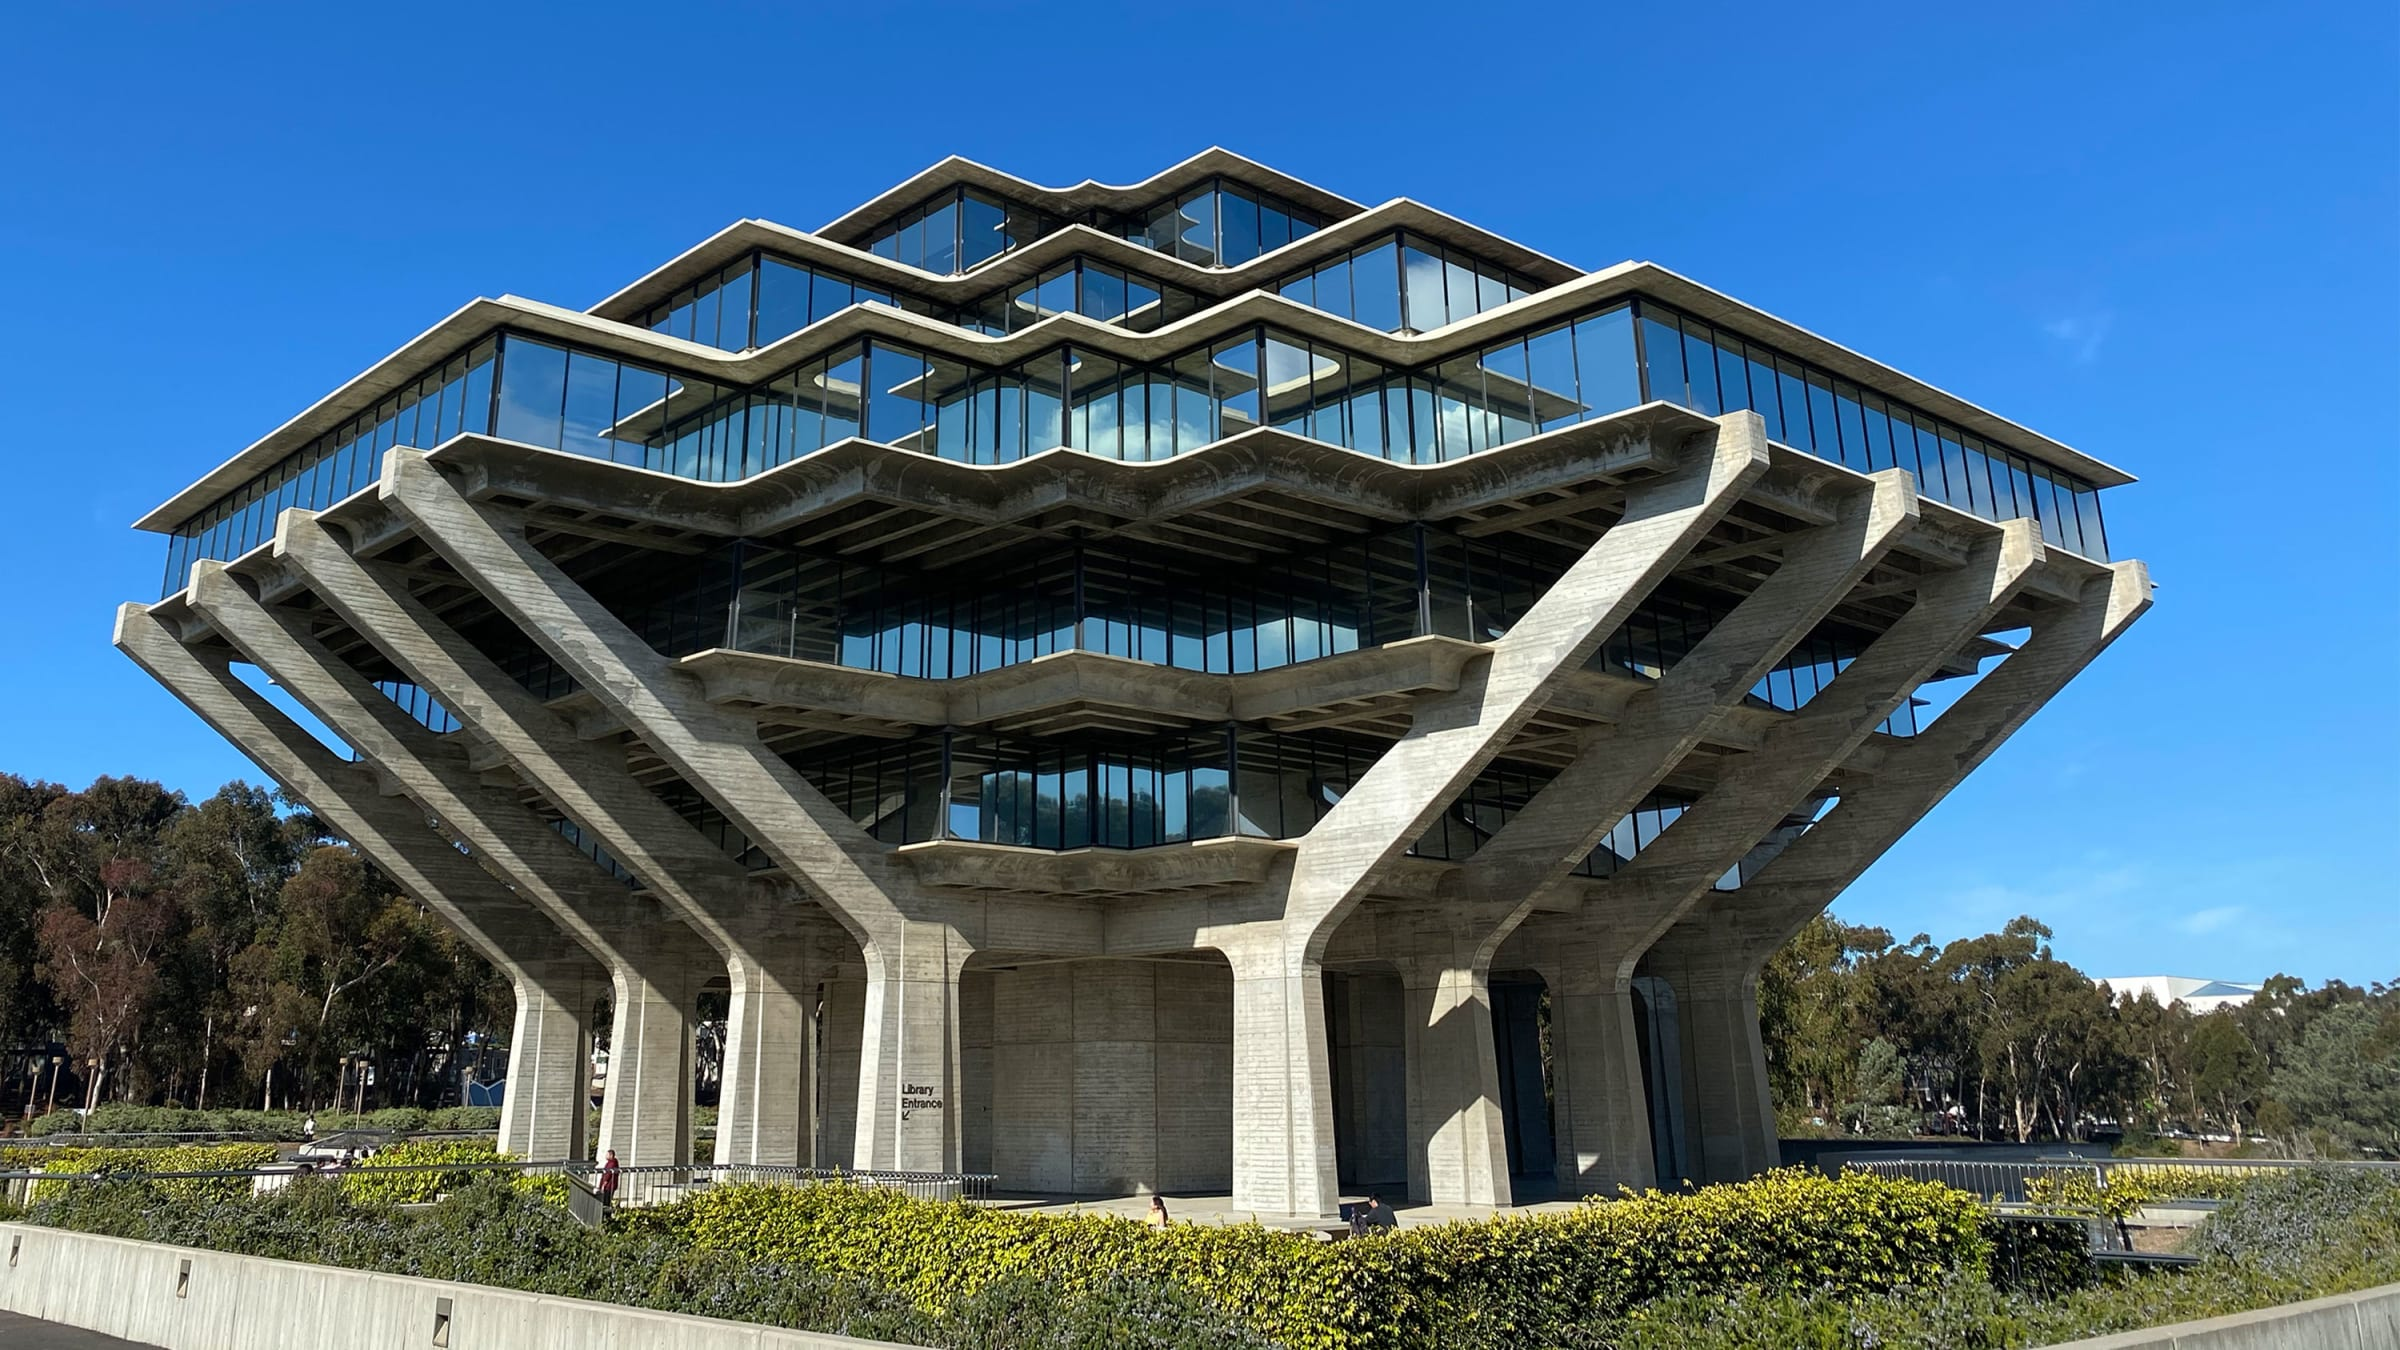
\includegraphics[width=.4\textwidth]{geisel.jpg} 
  \end{center}

    EXPLAIN your reasoning and EXPLAIN if you
    think your estimates are \textbf{too large} or \textbf{too small}
    in each case.
  \end{enumerate}
  
  \begin{freeResponse}
    \begin{enumerate}
    \item For the first statement, let's write our numbers as the
      product of a number between zero and one and a power of ten. So
      letting $a$ and $b$ be between $.1$ and $1$ we can write.
      \[
      \underbrace{a\cdot 10^m}_{\text{$m$-digit number}} + \underbrace{b\cdot 10^n}_{\text{$n$-digit number}}.
      \]
      Now write
      \begin{align*}
        a\cdot 10^m + b\cdot 10^n &= a\cdot 10^m + \frac{b}{10^{m-n}}\cdot 10^m \\
        &= 10^m \left(a +\frac{b}{10^{m-n}}\right).
      \end{align*}
      This will be a $m$-digit number, unless $a+\frac{b}{10^{m-n}}\ge 1$, in
      which case it will be a $(1+m)$-digit number.


      For the second statement, we start the same way
      \[
      \underbrace{a\cdot 10^m}_{\text{$m$-digit number}} \cdot \underbrace{b\cdot 10^n}_{\text{$n$-digit number}} = ab\cdot 10^{m+n}
      \]
      Now assume that $m\ge n$ and write
      \begin{align*}
        \left(a\cdot 10^m\right) \left(b\cdot 10^n\right)  &= (ab)10^m+n\\
      \end{align*}
      Note $ab<1$, and the smallest $ab$ can be is
      \[
      0.1\cdot 0.1 = .01.
      \]
      Hence our product will be a $(m+n)$-digit number unless $ab <
      0.1$. In that case it will be a $(m+n-1)$-digit number.
    \item From the Wikipedia page, we see that the tower has a height
      of $110$ feet and a diameter of $200$ feet. Since the tower is so lumpy, I'll estimate the volume as
      \[
      V = 110\cdot 110\cdot 110 = 1331000 \text{ cubic feet}.
      \]
      I believe this estimate is TOO LARGE.

      For the surface area I'll estimate
      \[
      SA = 6(200\cdot 200) = 240000\text{ square feet}.
      \]
      I believe this estimate is TOO SMALL, since the building is so very
      lumpy.
    \end{enumerate}
  \end{freeResponse}
\end{question}
\end{document}
